%<dscrpt>Fichier de déclarations Latex à inclure au début d'un élément de cours.</dscrpt>

\documentclass[a4paper]{article}
\usepackage[hmargin={1.8cm,1.8cm},vmargin={2.4cm,2.4cm},headheight=13.1pt]{geometry}

%includeheadfoot,scale=1.1,centering,hoffset=-0.5cm,
\usepackage[pdftex]{graphicx,color}
\usepackage[french]{babel}
%\selectlanguage{french}
\addto\captionsfrench{
  \def\contentsname{Plan}
}
\usepackage{fancyhdr}
\usepackage{floatflt}
\usepackage{amsmath}
\usepackage{amssymb}
\usepackage{amsthm}
\usepackage{stmaryrd}
%\usepackage{ucs}
\usepackage[utf8]{inputenc}
%\usepackage[latin1]{inputenc}
\usepackage[T1]{fontenc}


\usepackage{titletoc}
%\contentsmargin{2.55em}
\dottedcontents{section}[2.5em]{}{1.8em}{1pc}
\dottedcontents{subsection}[3.5em]{}{1.2em}{1pc}
\dottedcontents{subsubsection}[5em]{}{1em}{1pc}

\usepackage[pdftex,colorlinks={true},urlcolor={blue},pdfauthor={remy Nicolai},bookmarks={true}]{hyperref}
\usepackage{makeidx}

\usepackage{multicol}
\usepackage{multirow}
\usepackage{wrapfig}
\usepackage{array}
\usepackage{subfig}


%\usepackage{tikz}
%\usetikzlibrary{calc, shapes, backgrounds}
%pour la présentation du pseudo-code
% !!!!!!!!!!!!!!      le package n'est pas présent sur le serveur sous fedora 16 !!!!!!!!!!!!!!!!!!!!!!!!
%\usepackage[french,ruled,vlined]{algorithm2e}

%pr{\'e}sentation du compteur de niveau 2 dans les listes
\makeatletter
\renewcommand{\labelenumii}{\theenumii.}
\renewcommand{\thesection}{\Roman{section}.}
\renewcommand{\thesubsection}{\arabic{subsection}.}
\renewcommand{\thesubsubsection}{\arabic{subsubsection}.}
\makeatother


%dimension des pages, en-t{\^e}te et bas de page
%\pdfpagewidth=20cm
%\pdfpageheight=14cm
%   \setlength{\oddsidemargin}{-2cm}
%   \setlength{\voffset}{-1.5cm}
%   \setlength{\textheight}{12cm}
%   \setlength{\textwidth}{25.2cm}
   \columnsep=1cm
   \columnseprule=0.5pt

%En tete et pied de page
\pagestyle{fancy}
\lhead{MPSI-\'Eléments de cours}
\rhead{\today}
%\rhead{25/11/05}
\lfoot{\tiny{Cette création est mise à disposition selon le Contrat\\ Paternité-Pas d'utilisations commerciale-Partage des Conditions Initiales à l'Identique 2.0 France\\ disponible en ligne http://creativecommons.org/licenses/by-nc-sa/2.0/fr/
} }
\rfoot{\tiny{Rémy Nicolai \jobname}}


\newcommand{\baseurl}{http://back.maquisdoc.net/data/cours\_nicolair/}
\newcommand{\urlexo}{http://back.maquisdoc.net/data/exos_nicolair/}
\newcommand{\urlcours}{https://maquisdoc-math.fra1.digitaloceanspaces.com/}

\newcommand{\N}{\mathbb{N}}
\newcommand{\Z}{\mathbb{Z}}
\newcommand{\C}{\mathbb{C}}
\newcommand{\R}{\mathbb{R}}
\newcommand{\D}{\mathbb{D}}
\newcommand{\K}{\mathbf{K}}
\newcommand{\Q}{\mathbb{Q}}
\newcommand{\F}{\mathbf{F}}
\newcommand{\U}{\mathbb{U}}
\newcommand{\p}{\mathbb{P}}


\newcommand{\card}{\mathop{\mathrm{Card}}}
\newcommand{\Id}{\mathop{\mathrm{Id}}}
\newcommand{\Ker}{\mathop{\mathrm{Ker}}}
\newcommand{\Vect}{\mathop{\mathrm{Vect}}}
\newcommand{\cotg}{\mathop{\mathrm{cotan}}}
\newcommand{\sh}{\mathop{\mathrm{sh}}}
\newcommand{\ch}{\mathop{\mathrm{ch}}}
\newcommand{\argsh}{\mathop{\mathrm{argsh}}}
\newcommand{\argch}{\mathop{\mathrm{argch}}}
\newcommand{\tr}{\mathop{\mathrm{tr}}}
\newcommand{\rg}{\mathop{\mathrm{rg}}}
\newcommand{\rang}{\mathop{\mathrm{rg}}}
\newcommand{\Mat}{\mathop{\mathrm{Mat}}}
\newcommand{\MatB}[2]{\mathop{\mathrm{Mat}}_{\mathcal{#1}}\left( #2\right) }
\newcommand{\MatBB}[3]{\mathop{\mathrm{Mat}}_{\mathcal{#1} \mathcal{#2}}\left( #3\right) }
\renewcommand{\Re}{\mathop{\mathrm{Re}}}
\renewcommand{\Im}{\mathop{\mathrm{Im}}}
\renewcommand{\th}{\mathop{\mathrm{th}}}
\newcommand{\repere}{$(O,\overrightarrow{i},\overrightarrow{j},\overrightarrow{k})$}
\newcommand{\cov}{\mathop{\mathrm{Cov}}}

\newcommand{\absolue}[1]{\left| #1 \right|}
\newcommand{\fonc}[5]{#1 : \begin{cases}#2 \rightarrow #3 \\ #4 \mapsto #5 \end{cases}}
\newcommand{\depar}[2]{\dfrac{\partial #1}{\partial #2}}
\newcommand{\norme}[1]{\left\| #1 \right\|}
\newcommand{\se}{\geq}
\newcommand{\ie}{\leq}
\newcommand{\trans}{\mathstrut^t\!}
\newcommand{\val}{\mathop{\mathrm{val}}}
\newcommand{\grad}{\mathop{\overrightarrow{\mathrm{grad}}}}

\newtheorem*{thm}{Théorème}
\newtheorem{thmn}{Théorème}
\newtheorem*{prop}{Proposition}
\newtheorem{propn}{Proposition}
\newtheorem*{pa}{Présentation axiomatique}
\newtheorem*{propdef}{Proposition - Définition}
\newtheorem*{lem}{Lemme}
\newtheorem{lemn}{Lemme}

\theoremstyle{definition}
\newtheorem*{defi}{Définition}
\newtheorem*{nota}{Notation}
\newtheorem*{exple}{Exemple}
\newtheorem*{exples}{Exemples}


\newenvironment{demo}{\renewcommand{\proofname}{Preuve}\begin{proof}}{\end{proof}}
%\renewcommand{\proofname}{Preuve} doit etre après le begin{document} pour fonctionner

\theoremstyle{remark}
\newtheorem*{rem}{Remarque}
\newtheorem*{rems}{Remarques}

\renewcommand{\indexspace}{}
\renewenvironment{theindex}
  {\section*{Index} %\addcontentsline{toc}{section}{\protect\numberline{0.}{Index}}
   \begin{multicols}{2}
    \begin{itemize}}
  {\end{itemize} \end{multicols}}


%pour annuler les commandes beamer
\renewenvironment{frame}{}{}
\newcommand{\frametitle}[1]{}
\newcommand{\framesubtitle}[1]{}

\newcommand{\debutcours}[2]{
  \chead{#1}
  \begin{center}
     \begin{huge}\textbf{#1}\end{huge}
     \begin{Large}\begin{center}Rédaction incomplète. Version #2\end{center}\end{Large}
  \end{center}
  %\section*{Plan et Index}
  %\begin{frame}  commande beamer
  \tableofcontents
  %\end{frame}   commande beamer
  \printindex
}


\makeindex
\begin{document}
\noindent

\debutcours{Introduction aux systèmes linéaires}{1.0 \tiny{le \today} }

\section{Définitions}
\begin{defi}
Un système linéaire\index{système linéaire} de $n$ équations à $p$ inconnues est un système d'équations de la forme
\begin{displaymath}
 \left\lbrace 
\begin{aligned}
 a_{1,1}x_1 + a_{1,2}x_2 + \cdots + a_{1,p}x_p &= b_1\\
 a_{2,1}x_1 + a_{2,2}x_2 + \cdots + a_{2,p}x_p &= b_2\\
                                               &\vdots \\
 a_{n,1}x_1 + a_{n,2}x_2 + \cdots + a_{n,p}x_p &= b_n\\
\end{aligned}
\right. 
\end{displaymath}
où $x_1,\cdots x_p$ sont les inconnues. Lorsque les $a_{i,j}$ et les $b_k$ sont dans $\R$ ou $\C$, on dit que le système est à coefficients dans $\R$ ou $\C$.\newline Une solution est un élément de $(u_1,\cdots,u_p)\in\R^p$ ou $\C^p$ tel que
\begin{displaymath}
 \left\lbrace 
\begin{aligned}
 a_{1,1}u_1 + a_{1,2}u_2 + \cdots + a_{1,p}u_p &= b_1\\
 a_{2,1}u_1 + a_{2,2}u_2 + \cdots + a_{2,p}u_p &= b_2\\
                                               &\vdots \\
 a_{n,1}u_1 + a_{n,2}u_2 + \cdots + a_{n,p}u_p &= b_n\\
\end{aligned}
\right. 
\end{displaymath}
Un système est dit \emph{homogène}\index{système homogène} lorsque tous les $b_k$ sont nuls. Pour tout système, le système homogène associé est obtenu en gardant les mêmes $a_{i,j}$ et en prenant les $b_k$ nuls.\newline
Deux systèmes sont dits \emph{équivalents} \index{systèmes équivalents} si et seulement si ils ont le même ensemble de solutions.
\end{defi}
\begin{nota}
  Si on nomme un système particulier: par exemple $\mathcal{S}$, on convient souvent de noter $\mathcal{E}_{\mathcal{S}}$ l'ensemble des solutions. Le système $\mathcal{S}$ n'admet pas de solutions si et seulement si l'ensemble $\mathcal{E}_{\mathcal{S}}$ des solutions est vide.
\end{nota}

\begin{rem}
 Un système homogène à $p$ inconnues admet toujours la solution nulle $(0,\cdots,0)\in\R^p$ (ou $\C^p$).
\end{rem}

Deux questions principales se posent avec de tels systèmes.
\begin{enumerate}
 \item Pour un jeu de coefficients donné, le système admet-il des solutions? Plus précisément, pour un jeu de $a_{i,j}$ donné, peut-on former des conditions sur les $b_k$ caractérisant l'existence de solutions? Former de telles relations c'est \emph{éliminer} \index{éliminer} les inconnues du système.
 \item Si un système admet des solutions, comment décrire précisément l'ensemble des solutions?  Décrire l'ensemble de ses solutions en fonction de paramètres arbitraires c'est \emph{résoudre}\index{résoudre} un système.
\end{enumerate}
Exemples: caractériser que trois points sont alignés, ou quatre cocycliques.\newline
Trois points sont alignés si et seulement si ils sont contenus dans une droite. Considérons 3 points $A_1$, $A_2$, $A_3$ dans un plan muni d'un repère, leurs coordonnées sont respectivement
\[
 (x_1,y_1),\; (x_2,y_2),\; (x_3,y_3).
\]
Une droite est caractérisée par son équation c'est à dire qu'elle est formée par les points dont les ccordonnées $(x,y)$ vérifient
\[
 ax + by + c = 0 
\]
où $a, b, b$ sont des nombres réels $(a,b)\neq (0,0)$ fixés qui définissent la droite.\newline
On en déduit que $A_1, A_2, A_3$ sont alignés si et seulement si il existe $(a,b,c)$ réels avec $(a,b)\neq (0,0)$ tels que 
\[
 \left\lbrace
 \begin{aligned}
a x_1 + by_1 + c &= 0\\ a x_2 + by_2 + c &= 0\\ a x_3 + by_3 + c &= 0  
 \end{aligned}
\right.
\]
Autrement dit, les points $A_1,A_2,A_3$ sont alignés si et seulement si le système homogène $\mathcal{S}$ de 3 équations à 3 inconnues $u,v, w$ admet une solution $(a,b,c)$ telle $(a,b)\neq(0,0)$.
\[
 \mathcal{S}: \hspace{0.5cm}
 \left\lbrace
 \begin{aligned}
x_1u + y_1v + w &= 0\\ x_2u + y_2v + w &= 0\\ x_3u + y_3v + w &= 0  
 \end{aligned}
\right.
\]

Quelques idées fausses:
\begin{itemize}
 \item Un système avec plus d'équations que d'inconnues n'admet pas de solution (ou n'en admet qu'un nombre fini). Prendre, autant de fois que l'on veut, la même équation.
 \item Un système avec plus d'inconnues que d'équations admet toujours des solutions. Prendre une équation avec beaucoup d'inconnues, lui adjoindre une équation obtenue à partir de la première en changeant seulement le second membre. On obtient un système sans solution de deux équations avec beaucoup d'inconnues.
 \item Un système avec le même nombre d'équations que d'inconnues admet une solution unique. Un exemple montrant que c'est faux est facile à obtenir en combinant les deux idées précédentes.
\end{itemize}

\section{Propriétés de l'ensemble des solutions}
On note $\K$ le corps des coefficients c'est à dire $\R$ ou $\C$.
\begin{prop}
 Lorsqu'un système homogène à $p$ inconnues admet des solutions, l'ensemble des solutions (noté $\mathcal{E}$) est un sous-espace vectoriel de $\K^p$ c'est à dire que
\begin{displaymath}
 \forall (u_1,\cdots,u_p)\in \mathcal{E}, \forall (v_1,\cdots,v_p)\in \mathcal{E}, \forall \lambda \in \K:
  \left\lbrace 
\begin{aligned}
 &(u_1+v_1,\cdots,u_p+v_p)\in \mathcal{E}\\
 &\lambda(u_1,\cdots,u_p)= (\lambda u_1,\cdots,\lambda u_p)\in \mathcal{E}
\end{aligned}
\right. 
\end{displaymath}
\end{prop}
\begin{demo}
 \'Evident par linéarité. C'est à dire parce que les inconnues ne figurent qu'au premier degré et multipliées par des coefficients fixés.
\end{demo}
\begin{prop}
 Lorsqu'un système à $p$ inconnues admet une solution $u=(u_1,\cdots,u_p)$, l'ensemble (noté $\mathcal{E}$) de ses solutions vérifie
\begin{displaymath}
 \mathcal{E} = u + \mathcal{E}_0=\left\lbrace (u_1+v_1,\cdots,u_p+v_p)\text{ avec } (v_1,\cdots,v_p)\in \mathcal{E}_0\right\rbrace 
\end{displaymath}
où $\mathcal{E}_0$ est l'ensemble des solutions du système homogène associé.
\end{prop}
\begin{demo}
 Dans le système, remplaçons les seconds membres à l'aide de la solution particulière:
\begin{multline*}
 \left\lbrace 
\begin{aligned}
 a_{1,1}x_1 + a_{1,2}x_2 + \cdots + a_{1,p}x_p &= b_1\\
 a_{2,1}x_1 + a_{2,2}x_2 + \cdots + a_{2,p}x_p &= b_2\\
                                               &\vdots \\
 a_{n,1}x_1 + a_{n,2}x_2 + \cdots + a_{n,p}x_p &= b_n\\
\end{aligned}
\right. 
\Leftrightarrow 
 \left\lbrace 
\begin{aligned}
 a_{1,1}x_1 + a_{1,2}x_2 + \cdots + a_{1,p}x_p &= a_{1,1}u_1 + a_{1,2}u_2 + \cdots + a_{1,p}u_p\\
 a_{2,1}x_1 + a_{2,2}x_2 + \cdots + a_{2,p}x_p &= a_{2,1}u_1 + a_{2,2}u_2 + \cdots + a_{2,p}u_p\\
                                               &\vdots \\
 a_{n,1}x_1 + a_{n,2}x_2 + \cdots + a_{n,p}x_p &= a_{n,1}u_1 + a_{n,2}u_2 + \cdots + a_{n,p}u_p\\
\end{aligned}
\right. \\
\Leftrightarrow
 \left\lbrace 
\begin{aligned}
 a_{1,1}(x_1 - u_1) + a_{1,2}(x_2 - u_2) + \cdots + a_{1,p}(x_p - u_p) &= 0\\
 a_{2,1}(x_1 - u_1) + a_{2,2}(x_2 - u_2) + \cdots + a_{2,p}(x_p - u_p) &= 0\\
                                               &\vdots \\
 a_{n,1}(x_1 - u_1) + a_{n,2}(x_2 - u_2) + \cdots + a_{n,p}(x_p - u_p) &= 0\\
\end{aligned}
\right. \\
\Leftrightarrow (x_1 - u_1, x_2 - u_2, \cdots, x_p - u_p) \text{ solution de } \mathcal{S}_0
\Leftrightarrow \exists (v_1,\cdots,v_p) \in \mathcal{S}_0 \text{ tq }x_1 = u_1 + v_1, \cdots, x_p = u_p + v_p.
\end{multline*}

\end{demo}

\section{Opérations élémentaires}
\begin{figure}[ht]
 \centering
 \input{C9433_1.pdf_t}
 \caption{Procédure \og Nettoyer\fg}
 \label{fig:C9433_1}
\end{figure}

\begin{defi}\index{opérations élémentaires}
 Quatre opérations sur un système de $n$ équations à $p$ inconnues sont qualifiées d'\emph{élémentaires}.
\begin{itemize}
 \item Permuter deux lignes : codage $L_i\leftrightarrow L_j$.
 \item Permuter la place de deux inconnues dans toutes les lignes.
 \item Multiplier une ligne par un élément \emph{non nul} du corps: codage $L_i\leftarrow \lambda L_i$.
 \item Ajouter à une ligne une autre ligne multipliée par un élément du corps: codage $L_i\leftarrow L_i + \lambda L_j$.
\end{itemize}
\end{defi}
\begin{prop}
 Toute opération élémentaire transforme un système en un système équivalent.
\end{prop}
\begin{demo}
 Considérons un système $\mathcal{S}$ et $\mathcal{S}'$ le système obtenu par une opération élémentaire. Une solution de $\mathcal{S}$ est clairement encore solution de $\mathcal{S}'$. Cela se traduit par l'implication $\mathcal{S} \Rightarrow \mathcal{S}'$ entre les systèmes ou par l'inclusion $\mathcal{E}_S \subset \mathcal{E}_{S'}$ entre les ensembles de solutions.\newline
 En examinant les opérations élémentaires, on s'aperçoit que l'on peut aussi obtenir $\mathcal{S}$ en transformant $\mathcal{S}'$ par une opération élémentaire.\newline
 Par exemple si $\mathcal{S}'$ est obtenu à partir de $\mathcal{S}$ par la transformation codage $L_i\leftarrow L_i + \lambda L_j$ alors $\mathcal{S}$ est obtenu à partir de $\mathcal{S}'$ par la transformation codage $L_i\leftarrow L_i - \lambda L_j$.\newline
 Ceci assure que les ensembles de solutions sont les mêmes ou que les systèmes sont équivalents.
\end{demo}
L'algorithme du \emph{pivot de Gauss}\index{pivot de Gauss} combine les trois opérations élémentaires qui ne permutent pas les inconnues pour transformer le système en un système équivalent d'une forme particulière qui permet de répondre aux problématiques \og éliminer\fg~ et \og résoudre\fg.
\begin{figure}[h!t]
 \centering
 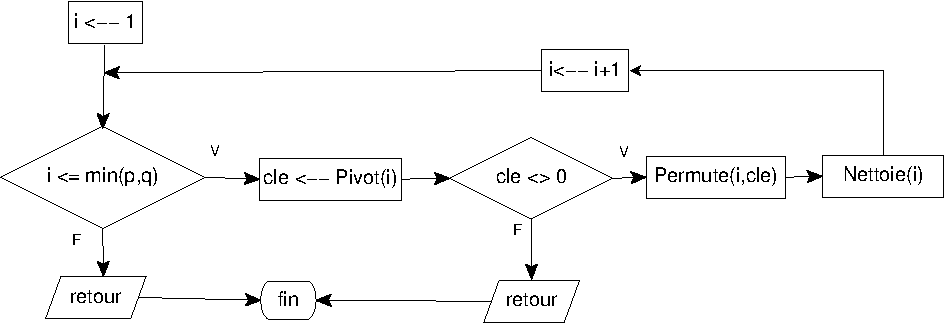
\includegraphics{C2234_1.pdf}
 \caption{Algorithme de Gauss}
 \label{fig:C2234_1}
\end{figure}

\section{Matrices et déterminants 2 x 2}
\index{matrices et déterminants!dimension 2} Applications aux systèmes.\newline
Une matrice $2\times2$ à coefficients réels est un tableau de quatre nombres
\begin{displaymath}
A=
 \begin{pmatrix}
  a & b \\
  c & d
 \end{pmatrix}
\end{displaymath}
L'ensemble des matrices $2\times2$ à coefficients réels est noté $\mathcal M_2(\R)$. On utilisera des parenthèses $( )$ ou des crochets $[ ]$ pour délimiter une matrice. La barre verticale est réservée au déterminant qui est un nombre attaché à une matrice.
\begin{displaymath}
 \det A =  \begin{vmatrix}
  a & b \\
  c & d
 \end{vmatrix}
= ad -bc
\end{displaymath}
Pour un traitement complet voir le chapitre \href{\baseurl C2261.pdf}{Déterminants}.
Les matrices et déterminants jouent un rôle capital dans l'étude des systèmes d'équations linéaires \index{système d'équations linéaires}. Ici on considère un système de deux équations à deux inconnues.
\begin{prop}Soit $a$, $b$, $c$, $d$, $u$, $v$ des nombres réels, le système linéaire $(\mathcal S)$ de deux équations aux deux inconnues $x$ et $y$ 
\begin{equation*}
 \left\lbrace 
\begin{aligned}
 a x + by &= u \\
 cx + dy &= v
\end{aligned}\right.  \qquad (\mathcal S)
\end{equation*}
admet un unique couple solution si et seulement le déterminant de la matrice associé est non nul. Lorsque ceci est réalisé, cet unique couple est :
\begin{displaymath}
 (\dfrac
{
\begin{vmatrix}
  u & b \\
  v & d
\end{vmatrix}
}
{
\begin{vmatrix}
  a & b \\
  c & d
\end{vmatrix}
} , 
\dfrac
{
\begin{vmatrix}
  a & u \\
  c & v
\end{vmatrix}
}
{
\begin{vmatrix}
  a & b \\
  c & d
\end{vmatrix}
}) \qquad \text{formules de Cramer}.
\end{displaymath}
\index{formules de Cramer}
\end{prop}
\begin{rem}
 Le couple solution est obtenu en remplaçant successivement chaque colonne de la matrice par la colonne du second membre.
\end{rem}
\begin{demo}
 \begin{itemize}
  \item Introduisons d'abord quelques notations 
\[
 D_1 =\begin{vmatrix}
  u & b \\
  v & d
\end{vmatrix}
 , \hspace{0.5cm}
 D_2 =\begin{vmatrix}
  a & u \\
  c & v
\end{vmatrix}
 , \hspace{0.5cm}
 D =\begin{vmatrix}
  a & b \\
  c & d
\end{vmatrix}.
\]

\item (analyse) Montrons d'abord que si $D\neq 0$ alors la \emph{seule solution possible} est donnée par les formules de Cramer. Supposons que $(x_0,y_0)$ soit un couple solution et remplaçons dans l'expression de $D_1)$.
\begin{displaymath}
 D_1 = ud-vb = (ax_0 + by_0)d-(cx_0+dy_0)b = D x_0 \Rightarrow x_0 = \dfrac{D_1}{D}
\end{displaymath}
Le calcul conduit à un résultat analogue pour $D_2$.

\item (synthèse) En remplaçant dans les équations, on obtient facilement que
\begin{displaymath}
 (\dfrac{D_1}{D}=\dfrac{1}{D}(ud-vb), \dfrac{D_2}{D}=\dfrac{1}{D}(av-cu))
\end{displaymath}
 est un couple solution.

\item Les deux derniers points montrent (analyse-synthèse) que lorsque $D\neq0$ le système admet une unique solution donnée par les formules de Cramer.

\item Montrons maintenant que si le système admet une unique solution alors $D\neq 0$. En fait on va plutôt montrer que si $D=0$ alors le système admet plusieurs solutions ou n'en admet aucune.\newline
Supposons que $D=0$ et que $(x_0,y_0)$ soit une solution. Considérons pour tout réel $\lambda$ :
\[
 x_\lambda = x_0 -\lambda b, \hspace{0.5cm} y_\lambda = y_0 +\lambda a.
\]
Il est alors évident par définition que $ax_\lambda + by_\lambda =u$. De plus :
\begin{displaymath}
 cx_\lambda + dy_\lambda = v +\lambda(-cb+ad) = v.
\end{displaymath}
On a donc obtenu une infinité de solutions.
\end{itemize}
\end{demo}

Ces résultats sont utilisés dans l'étude des \href{\baseurl C1616.pdf}{équations différentielles linéaires} ainsi que dans la \href{\baseurl C2005.pdf}{géométrie élémentaire du plan}. Leur signification en termes d'intersections de droites est si claire qu'elle rend presque inutile une démonstration. Celle proposée ici permet de mettre en pratique un peu de logique.

\end{document}
